\documentclass{article}%
\usepackage[T1]{fontenc}%
\usepackage[utf8]{inputenc}%
\usepackage{lmodern}%
\usepackage{textcomp}%
\usepackage{lastpage}%
\usepackage{authblk}%
\usepackage{graphicx}%
%
\title{Mutation of the Diamond{-}Blackfan Anemia Gene Rps7 in Mouse Results in Morphological and Neuroanatomical Phenotypes}%
\author{Brian Keller}%
\affil{Department of Biology and Biochemistry and the Centre for Regenerative Medicine, University of Bath, Bath, United Kingdom, \newline%
    Department of Pharmacy and Pharmacology and the Centre for Regenerative Medicine, University of Bath, Bath, United Kingdom}%
\date{01{-}01{-}2012}%
%
\begin{document}%
\normalsize%
\maketitle%
\section{Abstract}%
\label{sec:Abstract}%
(LabResults)\newline%
TPM1 is a DNA molecule that carries genetic information that can be understood to be identical to that of a single copy of its DNA base, but carries different genetic information in its other copies. TPM1 is a key component of the epigenetic and epigenetic structures necessary for the regulation of DNA methylation. These epigenetic and epigenetic structures undergo development in the non{-}genetic context, creating marked differences in DNA methylation in the macrophages, the cells messenger cells.\newline%
Inhibition of these epigenetic regulatory mechanisms may lead to the development of cancer. The epigenetic and epigenetic structures of human leukocytes promote the differentiation of various types of cancer cells based on those of other cancer cells. Each type of cancer cell forms unique epigenetic groups. In the case of cancer, the abnormal response to chemotherapy causes the leukemia cells to drift away from this conformational group.\newline%
While we know for certain that these new protein expression complexes are involved in the disease process, we are uncertain about their therapeutic benefit. There are two possible reasons for this uncertainty. Either these protein complex complexes inhibit the growth of cancer cells, or they may indirectly affect the growth and development of these types of cancer cells. In this connection, the interpretation of the findings in diabetic cell lines of monoclonal antibody{-}induced protein complexes involving TPM1 may give us a clue as to whether these complex complexes may be able to affect the disease process at the genetic level.

%
\subsection{Image Analysis}%
\label{subsec:ImageAnalysis}%


\begin{figure}[h!]%
\centering%
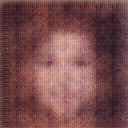
\includegraphics[width=150px]{500_fake_images/samples_5_470.png}%
\caption{A Man In A Black Shirt And A Black Tie}%
\end{figure}

%
\end{document}